\subsection{Dimension 1: Task completion rate and token efficiency}

\subsubsection{Setup}
\paragraph{Agents and Models.}
The experiments compare a small set of representative agent systems and backbone models:
\begin{itemize}
    \item \textbf{Agents.} GenericAgent (GA), Claude Code, OpenClaw, and Codex.
    \item \textbf{Models.} Claude Sonnet 4.6, Claude Opus 4.6, Minimax M2.7, and GPT-5.4.
\end{itemize}


\paragraph{Benchmark.}
We evaluate the systems on three benchmarks that cover complementary task structures:
\begin{itemize}
    \item \textbf{SOP-Bench.} An industrial SOP-following benchmark with multi-step order-fulfillment tasks. Agents must follow explicit procedural constraints, invoke multiple tools in the correct order, and complete the full execution chain from verification to final fulfillment decisions.
    \item \textbf{Lifelong AgentBench.} A sequential task benchmark designed to test continual capability accumulation. In the reported setting, the benchmark contains database-operation tasks with cross-task dependency, requiring the agent to maintain state, reuse prior discoveries, and complete tasks under strict execution order.
    \item \textbf{RealFin-benchmark.} A financial-task benchmark with 20 realistic tasks spanning indicator screening, correlation analysis, volatility ranking, price-volume pattern discovery, and structured result generation. The benchmark emphasizes domain understanding, code execution stability, and correct end-to-end completion.
\end{itemize}

\paragraph{Evaluations.}
Following the original experiment protocol:
\begin{itemize}
    \item \textbf{Accuracy.} The proportion of correctly solved tasks under each benchmark's verification protocol.
    \item \textbf{Input / Output / Total Tokens.} The reported token-cost statistics for each agent setting.
    \item \textbf{Token Efficiency.} Accuracy / (Total Tokens in Millions).
\end{itemize}
All systems are run on the same task sets with per-task execution and independently saved outputs.



\subsubsection{Results}

\begin{table*}[htbp]
\centering
\caption{\textbf{Task completion rate and token efficiency across the main agent benchmarks and RealFin-benchmark.} Each block reports the original metrics used in the corresponding benchmark. Since the efficiency ratio is normalized with different token scales across benchmarks, its absolute values should only be compared within the same benchmark block.}
\def\arraystretch{0.99}
\setlength{\tabcolsep}{0.45em}
\resizebox{1.0\linewidth}{!}{
\begin{tabular}{llccccc}
\toprule
\textbf{Agent} & \textbf{Model} & \textbf{Accuracy} & \textbf{Input Tokens} & \textbf{Output Tokens} & \textbf{Total Tokens} & \textbf{Efficiency} \\
\midrule
\rowcolor{bgcolor}
\multicolumn{7}{c}{\textbf{SOP-Bench}} \\
GA & Claude Sonnet 4.6 & 100\% & 2.02M & 53k & 2.08M & 0.48 \\
OpenClaw & Claude Sonnet 4.6 & 100\% & 2.60M & 40k & 2.64M & 0.38 \\
Claude Code & Claude Sonnet 4.6 & 85\% & 1.23M & 23k & 1.25M & 0.68 \\
GA & Minimax M2.7 & 90\% & 893k & 32k & 924k & 0.97 \\
OpenClaw & Minimax M2.7 & 95\% & 2.91M & 46k & 2.96M & 0.32 \\
\midrule
\rowcolor{bgcolor}
\multicolumn{7}{c}{\textbf{Lifelong AgentBench}} \\
GA & Claude Sonnet 4.6 & 100\% & 222k & 20k & 241k & 4.15 \\
OpenClaw & Claude Sonnet 4.6 & 70\% & 1.43M & 21k & 1.45M & 0.48 \\
Claude Code & Claude Sonnet 4.6 & 75\% & 800k & 14k & 814k & 0.92 \\
GA & Minimax M2.7 & 90\% & 400k & 23k & 423k & 2.12 \\
OpenClaw & Minimax M2.7 & 70\% & 1.20M & 17k & 1.22M & 0.57 \\
\midrule
\rowcolor{bgcolor}
\multicolumn{7}{c}{\textbf{RealFin-benchmark}} \\
GA & Claude Sonnet 4.6 & 65\% & 102k & 12k & 114k & 5.70 \\
Claude Code & Claude Opus 4.6 & 60\% & 290k & 17k & 307k & 1.95 \\
Claude Code & Claude Sonnet 4.6 & 55\% & 226k & 12k & 238k & 2.31 \\
OpenClaw & Claude Sonnet 4.6 & 35\% & 249k & 2k & 115k & 3.04 \\
Codex & GPT-5.4 & 60\% & 838k & 54k & 892k & 0.67 \\
\bottomrule
\end{tabular}
}
\label{tab:dimension1_task_completion}
\end{table*}

\textbf{GA maintains leading or near-leading task completion across different benchmarks.}
This trend is consistent across SOP-Bench, Lifelong AgentBench, and RealFin-benchmark. On the Claude-based runs, GA achieves 100\% accuracy on both SOP-Bench and Lifelong AgentBench, matching the best result on SOP-Bench and outperforming all baselines on Lifelong AgentBench. A similar pattern is observed on RealFin-benchmark, where GA attains the highest accuracy of 65\%, exceeding Claude Code Opus and Codex (60\%), Claude Code Sonnet (55\%), and OpenClaw (35\%).

\textbf{GA requires fewer tokens to complete tasks, especially in terms of input tokens.}
On SOP-Bench, GA uses 2.02M input tokens, which is lower than OpenClaw (2.60M) but higher than Claude Code (1.23M), while still achieving 100\% accuracy. In contrast, on Lifelong AgentBench, GA uses 222k input tokens, significantly lower than Claude Code (800k) and OpenClaw (1.43M), while maintaining 100\% accuracy. A similar pattern is observed on RealFin-benchmark.

\textbf{GA achieves the best trade-off between task completion and token cost across benchmarks.}
On SOP-Bench, Claude Code shows a higher efficiency ratio only at the cost of reduced accuracy (85\% vs. 100\%), whereas GA maintains full completion. On Lifelong AgentBench, GA achieves both the highest accuracy and the highest efficiency ratio (4.15), outperforming Claude Code (0.92) and OpenClaw (0.48). On RealFin-benchmark, GA again provides the best trade-off, reaching 65\% accuracy with 114k total tokens, corresponding to an efficiency ratio of 5.70, compared to 2.31 for Claude Code Sonnet, 1.95 for Claude Code Opus, 3.04 for OpenClaw, and 0.67 for Codex.


\subsection{Dimension 3: Self-Evolution Capability}
\label{sec:self_evolution_capability}

\subsubsection{Setup}
\paragraph{Task and Setting.}
We evaluate GA's self-evolution process in two complementary settings. The first is a nine-round longitudinal study on a LangChain GitHub research task that requires identifying the five most recently merged bug-related PRs, tracing their linked issues to extract the underlying modules, and verifying from the LangChain documentation whether these modules have troubleshooting guidance. The second is an eight-task web benchmark used to test whether the same SOP-driven efficiency gains transfer across task types. The longitudinal study exposes the full evolution trajectory from first execution to convergence, while the benchmark study tests whether the resulting efficiency pattern generalizes beyond a single workflow.

\paragraph{Evolution Stages.}
We find that GA's self-evolution process can be summarized into three recurring stages, each corresponding to a different level of experience compression and execution efficiency. We therefore evaluate the system's performance across these three stages.
\begin{itemize}
    \item \textbf{Stage 1: Natural-language execution.} GA first operates in an exploratory regime, where the task is solved mainly through in-context reasoning and trial-and-error interaction.
    \item \textbf{Stage 2: SOP distillation.} The accumulated experience is then compressed into a textual SOP, which reduces repeated exploration but still requires runtime interpretation and task-specific adaptation.
    \item \textbf{Stage 3: Code-based execution.} Finally, the verified workflow is codified into executable logic, so the agent can reuse the learned procedure with minimal LLM involvement.
\end{itemize}
\paragraph{Evaluations.}
\begin{itemize}
    \item \textbf{Time.} End-to-end wall-clock runtime for each execution.
    \item \textbf{LLM Calls.} Total number of model invocations per run.
    \item \textbf{Input / Output / Cache Tokens.} Token cost broken down into prompt input, model output, cache creation, and cache reading where available.
    \item \textbf{Total Tokens.} Aggregate token cost per run.
    \item \textbf{Reduction Ratio.} Relative decrease against the first execution in the longitudinal study, or against the no-SOP baseline in the cross-task benchmark.
\end{itemize}

\subsubsection{Iteration-Wise Efficiency Trajectory}

\begin{table*}[htbp]
\centering
\caption{\textbf{Nine-round evolution trajectory on the LangChain GitHub research task.} The experiment starts from scratch in Round \#1, iteratively refines a textual SOP in Rounds \#2--\#5, and enters the codified execution regime in Rounds \#6--\#9.}
\def\arraystretch{0.99}
\setlength{\tabcolsep}{0.42em}
\resizebox{1.0\linewidth}{!}{
\begin{tabular}{l l c c c c c c c}
\toprule
\textbf{Round} & \textbf{Stage} & \textbf{Time} & \textbf{LLM Calls} & \textbf{Input} & \textbf{Output} & \textbf{Cache Create} & \textbf{Cache Read} & \textbf{Total} \\
\midrule

\#1 & Initial run & 7m30s & 32 & 15,581 & 7,647 & 15,600 & 183,375 & 222,203 \\
\#2 & SOP optimization & 4m19s & 12 & 5,045 & 4,860 & 4,553 & 51,883 & 66,341 \\
\#3 & SOP optimization & 2m53s & 8 & 2,538 & 4,598 & 3,155 & 39,534 & 49,825 \\
\#4 & SOP optimization & 2m29s & 9 & 3,265 & 3,682 & 3,435 & 41,376 & 51,758 \\
\#5 & SOP optimization & 2m50s & 7 & 2,568 & 3,276 & 2,424 & 27,268 & 35,536 \\
\#6 & Codified SOP & 2m24s & 6 & 1,855 & 1,064 & 1,930 & 20,913 & 25,762 \\
\#7 & Codified SOP & 1m41s & 5 & 1,931 & 1,126 & 1,708 & 18,249 & 23,014 \\
\#8 & Codified SOP & 1m35s & 5 & 1,884 & 990 & 1,586 & 18,229 & 22,689 \\
\#9 & Codified SOP & 1m38s & 5 & 1,323 & 994 & 1,659 & 19,034 & 23,010 \\

\bottomrule
\end{tabular}
}
\label{tab:self_evolution_rounds}
\end{table*}

\textbf{The nine-round trajectory shows a phase transition from high-entropy exploration to a stable low-cost execution regime.} Relative to Round \#1, the final execution in Round \#9 reduces runtime from 7m30s to 1m38s (78.2\%), LLM calls from 32 to 5 (84.4\%), and total tokens from 222,203 to 23,010 (89.6\%). The key pattern is not just the large first-to-last gap, but the structure of the transition itself. During the textual SOP stage, token cost follows a non-monotonic but downward path (66k $\rightarrow$ 50k $\rightarrow$ 52k $\rightarrow$ 36k), which suggests that SOP compression already removes most redundant exploration, while still paying an adaptation cost whenever the stored procedure must be aligned with newly encountered edge cases. Once the workflow is codified, the system enters a narrow convergence band of roughly 23k$\pm$1k tokens across Rounds \#6--\#9, indicating that execution has become predictable rather than exploratory.

\textbf{Most of the efficiency gain comes from eliminating repeated reasoning cycles rather than merely shortening individual responses.} The dominant change is the collapse in call count, which removes entire understand--reason--generate loops from the execution trace. This is consistent with the token composition: cache-read tokens fall from 183,375 in Round \#1 to 19,034 in Round \#9, and input tokens fall from 15,581 to 1,323, showing that the agent no longer rebuilds large amounts of context at runtime. Per-call token load also drops substantially over the course of evolution, from 6,944 tok/call in Round \#1 to about 4.5k--4.6k tok/call in Rounds \#7--\#9, but this effect is secondary to the structural reduction in the number of calls. The larger implication is that textual SOPs already compress the search space, while code-level execution removes the remaining interpretation overhead and turns the learned workflow into a deterministic asset.

\subsubsection{Cross-Task Efficiency Gains}
\begin{figure*}[htbp]
\centering
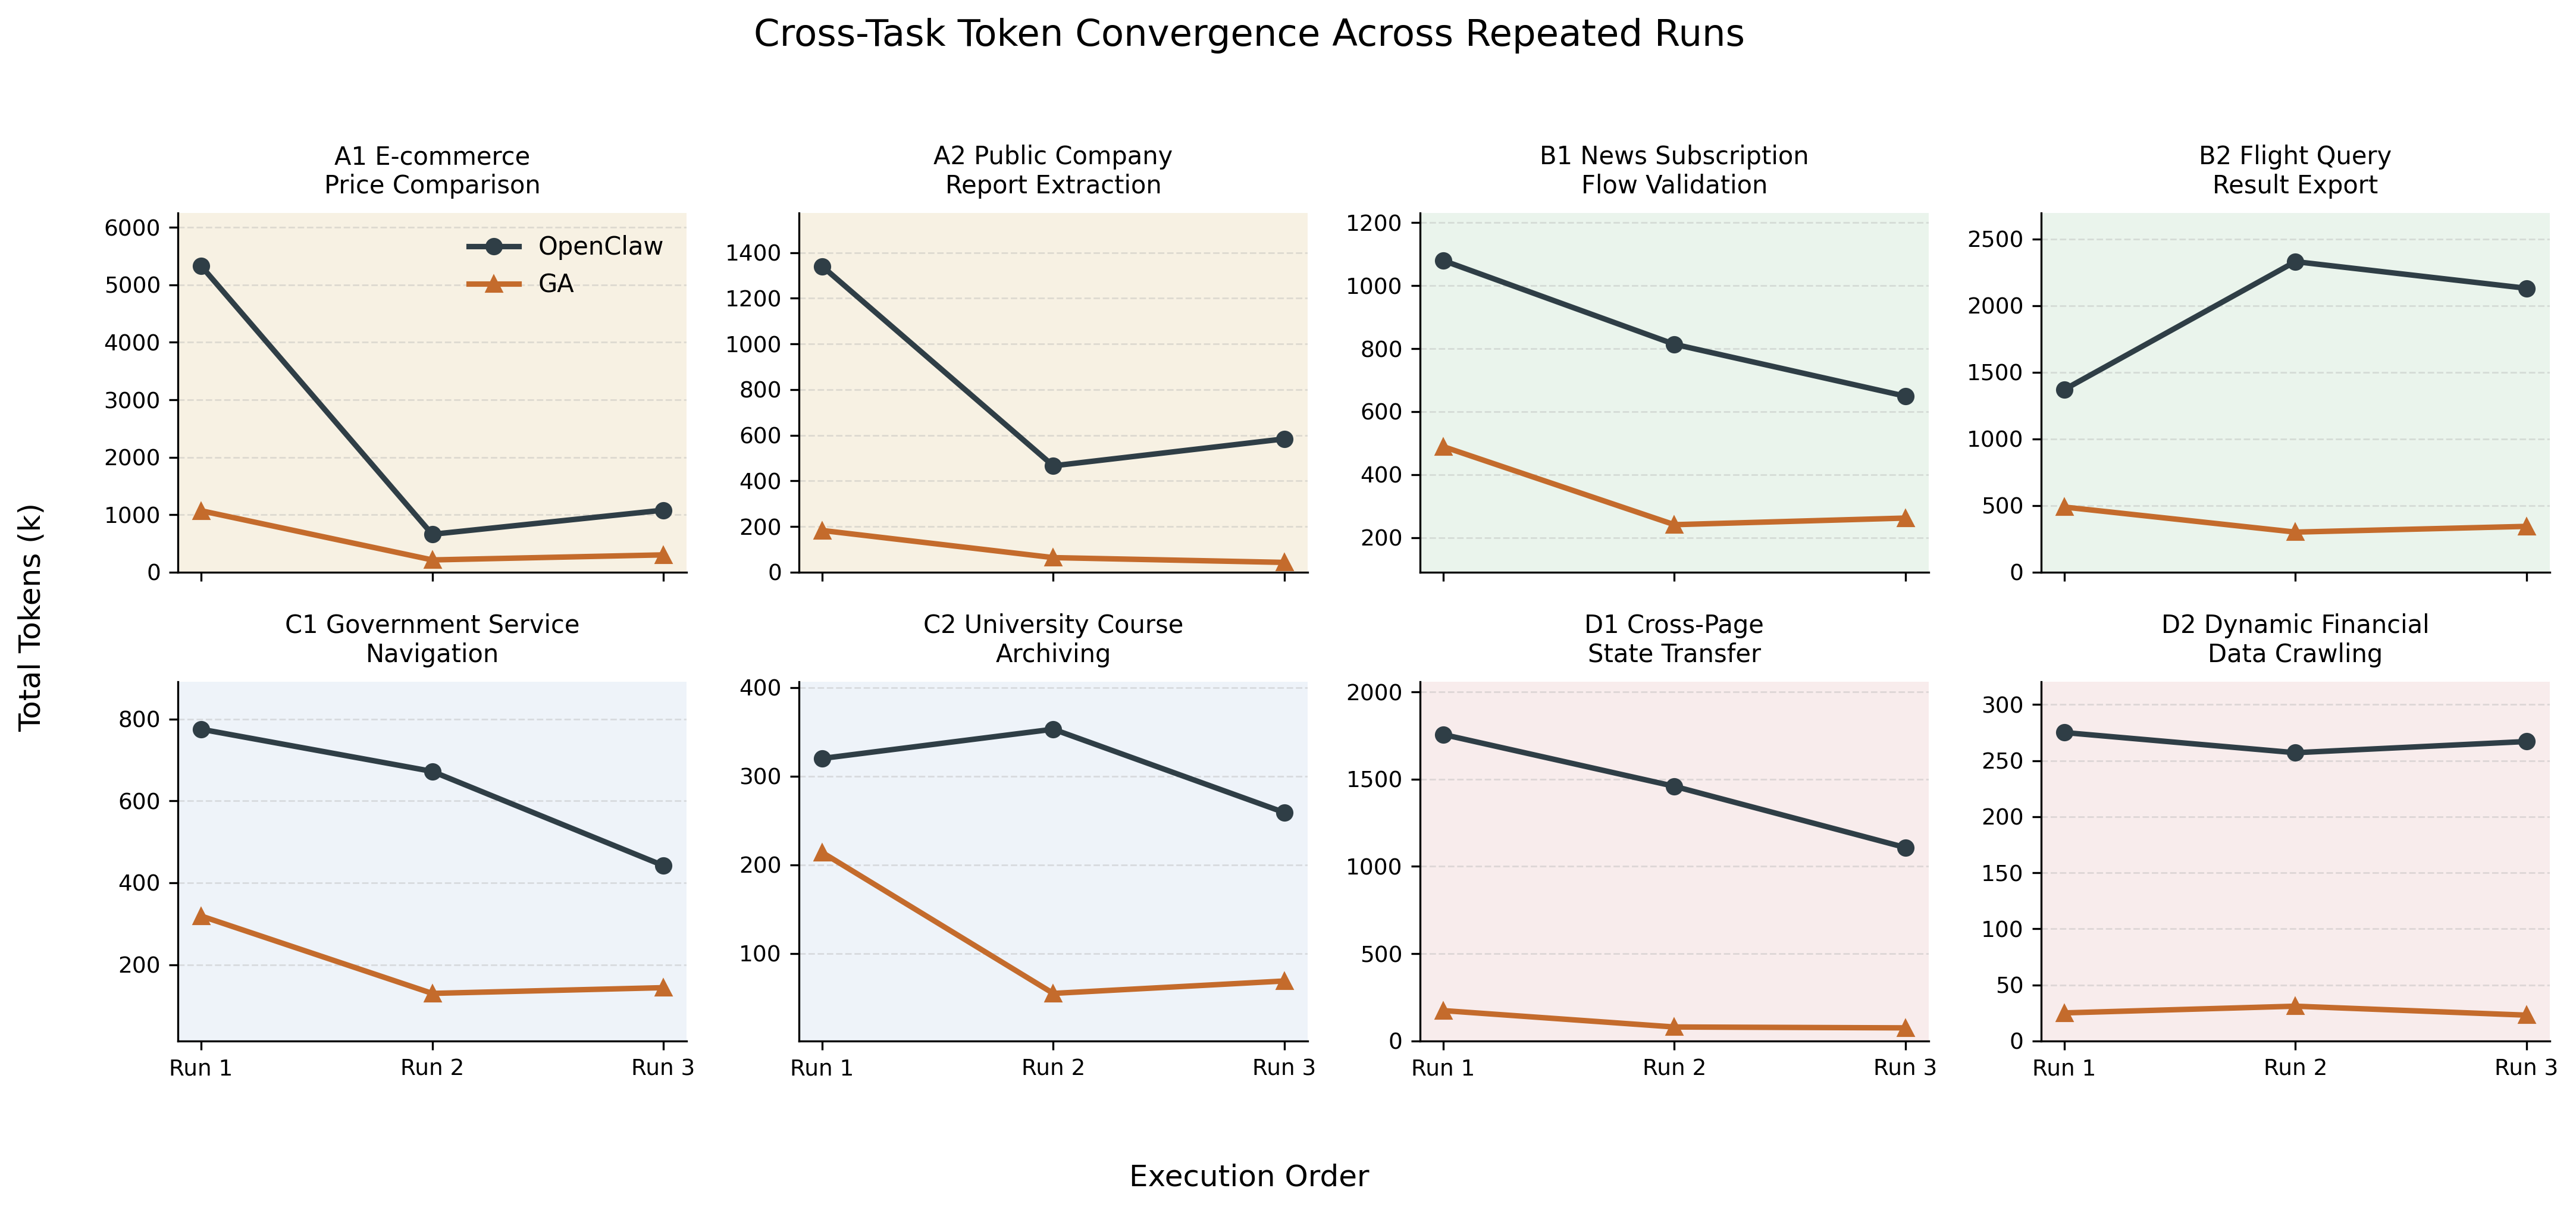
\includegraphics[width=0.9\linewidth]{image/cross_task_convergence.png}
\caption{\textbf{Cross-task token convergence across repeated runs for OpenClaw and GA.} Each panel corresponds to one benchmark task and plots total token consumption over the first, second, and third executions. GA shows a consistent ``cold start + rapid convergence'' pattern: token cost is typically highest on the first run, then quickly drops and stabilizes in later runs. In contrast, OpenClaw usually remains flat or unstable across repetitions, indicating that it continues to re-explore the task instead of reusing prior experience. The gap is especially large on long-horizon dependency tasks, where SOP reuse brings the strongest efficiency gains. The figure was generated from the benchmark data using \texttt{self-evo/plot\_cross\_task\_convergence.py}.}
\label{fig:cross_task_convergence}
\end{figure*}
\textbf{The efficiency gains transfer across tasks rather than remaining confined to a single hand-optimized workflow.} On all eight benchmark tasks, GA consumes fewer tokens than the no-memory baseline, with savings ranging from 61.0\% to 92.4\% and an overall reduction of 79.3\%. This consistency matters more than any individual best case: it shows that SOP self-evolution is not just memorizing one task, but systematically converting prior successful trajectories into reusable execution shortcuts. The strongest gains appear in long-horizon tasks with state transfer and recovery (Category D, 92.0\%), where repeated failure handling and path search dominate the baseline cost. In those cases, SOP acts as path compression: once the verified route is stored, the agent can bypass most exploratory branches entirely.

\textbf{GA exhibits a clear ``cold start + rapid convergence'' pattern across repeated executions of the same task.} Looking at the three runs of each benchmark task, GA shows the same internal trend: the first run has substantially higher token cost, while the second and third runs quickly converge to a stable low-cost regime. This indicates that even with SOP memory, the first execution still incurs an SOP adaptation cost, because the agent must map generalized SOP knowledge onto the concrete page structure and interaction flow of the current task instance. However, this adaptation happens only once. After the successful path is aligned with the environment, later executions can directly reuse that result and rapidly drop to a stable token level. By contrast, OpenClaw shows no comparable convergence pattern across its three runs. On B2, for example, token usage changes from 1,370k to 2,330k to 2,130k, which means the system keeps re-exploring rather than reusing prior experience. This distinction is important for deployment: GA pays a one-time adaptation cost on a new task, but its marginal cost quickly approaches zero, whereas the baseline remains expensive on every execution.

\textbf{The benefit of SOP memory tends to increase with task complexity.} When the tasks are ordered by OpenClaw's average token consumption as a proxy for intrinsic task complexity, a positive relationship emerges between complexity and saving rate. High-complexity tasks with OC averages above 1,000k tokens, such as A1, B2, and D1, achieve an average saving of 83.5\%, while mid-complexity tasks average 72.5\%. Although D2 is low in absolute token cost, its 90.1\% saving rate is consistent with the same mechanism because it still contains long-horizon dependency structure. The broader implication is that SOP self-evolution becomes more valuable as tasks require more multi-step reasoning, navigation, and recovery from branching execution paths: in simple tasks it is helpful, but in complex tasks it becomes structurally decisive.

\subsection{Dimension 4: Tool-use efficiency}
\label{sec:dimension4_tool_use_efficiency}

\subsubsection{Setup}
\paragraph{Baseline.}
All compared systems use the same backbone model, Claude Sonnet 4.6. We evaluate three representative tool-use designs:
\begin{itemize}
    \item \textbf{GA.} A minimal atomic-tool design that relies on a small set of general-purpose tools and solves downstream tasks through tool composition.
    \item \textbf{Claude Code.} A strong baseline with a richer specialized tool ecosystem, used to test whether GA can match specialized tool capability without relying on tool-name alignment.
    \item \textbf{OpenClaw.} A multi-tool agent with several specialized or environment-dependent tool capabilities, used to compare tool-use efficiency and stability under a less minimal design.
\end{itemize}

\paragraph{Basic Tool Alignment.}
We align the systems at the capability level rather than at the tool-name level. The first column defines the target capability category, and the remaining three columns list the corresponding tool or mechanism used by each system to realize that capability.
\begin{table*}[htbp]
\centering
\caption{\textbf{Capability-level alignment of the basic tooling environment.} Each row maps one capability category to the corresponding tool in Claude Code, OpenClaw, and GA.}
\def\arraystretch{0.99}
\setlength{\tabcolsep}{0.42em}
\resizebox{1.0\linewidth}{!}{
\begin{tabular}{llll}
\toprule
\textbf{Capability Category} & \multicolumn{3}{c}{\textbf{Corresponding Tool / Mechanism}} \\
\cmidrule(lr){2-4}
 & \textbf{Claude Code} & \textbf{OpenClaw} & \textbf{GA} \\
\midrule
Code execution & BashTool & exec / process / nodes & code\_run \\
File reading & FileReadTool & read & file\_read \\
File writing & FileWriteTool & write & file\_write \\
Local file editing & FileEditTool & write / patch-like editing & file\_patch \\
Web reading  & WebFetchTool / browser read & browser base reading & web\_scan \\
Web interaction & WebBrowserTool / browser actions & browser interaction & web\_execute\_js \\
Working memory & TodoWriteTool / BriefTool & session history / status-like ability & update\_working\_checkpoint \\
\bottomrule
\end{tabular}
}
\label{tab:tooluse_basic_alignment}
\end{table*}

\paragraph{Benchmark.}
The benchmark contains two complementary task groups:
\begin{itemize}
    \item \textbf{Simple tool-generalization tasks.} These tasks test whether baseline specialized tool capabilities can be reproduced through GA's atomic-tool composition. The reported main set contains six Claude-Code-oriented tasks and five OpenClaw-oriented tasks whose intended baseline capability match is stable.
    \item \textbf{Long-horizon complex tasks.} These tasks test whether the same minimal tool design remains effective on realistic multi-step workflows, including document generation, SQL query generation, experiment analysis, procurement decision-making, and paper-reproduction feasibility analysis.
\end{itemize}

\paragraph{Metrics.}
\begin{itemize}
    \item \textbf{Task Success.} Whether the task passes evaluation.
    \item \textbf{Task Completion Score.} Degree of completion on a 0--1 scale.
    \item \textbf{Request Count.} Number of agent--model interaction requests.
    \item \textbf{Tool Call Count.} Number of tool invocations.
    \item \textbf{Distinct Tool Count.} Number of different tools used in a task.
    \item \textbf{Distinct Capability Count.} Number of different capability categories exercised in a task.
    \item \textbf{Accounted Tokens.} Unified token cost defined as input + output + cache-read + cache-write tokens.
\end{itemize}

\subsubsection{Atomic Tool Generalization}

\begin{table*}[htbp]
\centering
\caption{\textbf{Aggregated results on long-horizon complex tasks.} This table reports the average outcomes over the long-horizon task set rather than expanding into per-task detail.}
\def\arraystretch{0.99}
\setlength{\tabcolsep}{0.42em}
\resizebox{1.0\linewidth}{!}{
\begin{tabular}{lccccccc}
\toprule
\textbf{Agent} & \textbf{\#Tasks} & \textbf{Success} & \textbf{Accounted Tokens} & \textbf{Time (s)} & \textbf{Requests} & \textbf{Tool Calls} & \textbf{Distinct Tools / Caps.} \\
\midrule
Claude Code & 5 & 100.0\% & 537,413 & 320.8 & 32.6 & 22.6 & 4.4 / 3.8 \\
GA & 5 & 100.0\% & 188,829 & 220.8 & 11.0 & 12.8 & 3.6 / 3.6 \\
OpenClaw & 5 & 80.0\% & 633,101 & 183.1 & 15.0 & 16.6 & 4.2 / 3.2 \\
\bottomrule
\end{tabular}
}
\label{tab:tooluse_long_horizon}
\end{table*}

\textbf{GA can solve complex long-horizon tasks through compositions of atomic tools rather than through a richer specialized tool inventory.} In Table~\ref{tab:tooluse_long_horizon}, GA reaches 100\% success on the five long-horizon tasks, matching Claude Code and outperforming OpenClaw, which falls to 80\%. This shows that a minimal tool set does not weaken capability reachability when the tools are composable in the right way. We provide more detailed empirical analyses of concrete atomic-tool compositions in the appendix, where simpler replacement cases offer additional evidence for the same capability-generalization claim.

\textbf{GA reduces token overhead while preserving task performance.} Although it matches Claude Code on success, GA uses only 188,829 accounted tokens, which is 35.1\% of Claude Code's 537,413 and 29.8\% of OpenClaw's 633,101. The same pattern appears in the interaction trace: GA reduces requests from 32.6 to 11.0 and tool calls from 22.6 to 12.8 relative to Claude Code, while OpenClaw remains both less stable and more expensive. The result indicates that GA's advantage comes from lower context and tool-process overhead, not from sacrificing quality.



\subsubsection{Dimension-Wise Tool Efficiency Comparison}

\begin{figure*}[htbp]
\centering
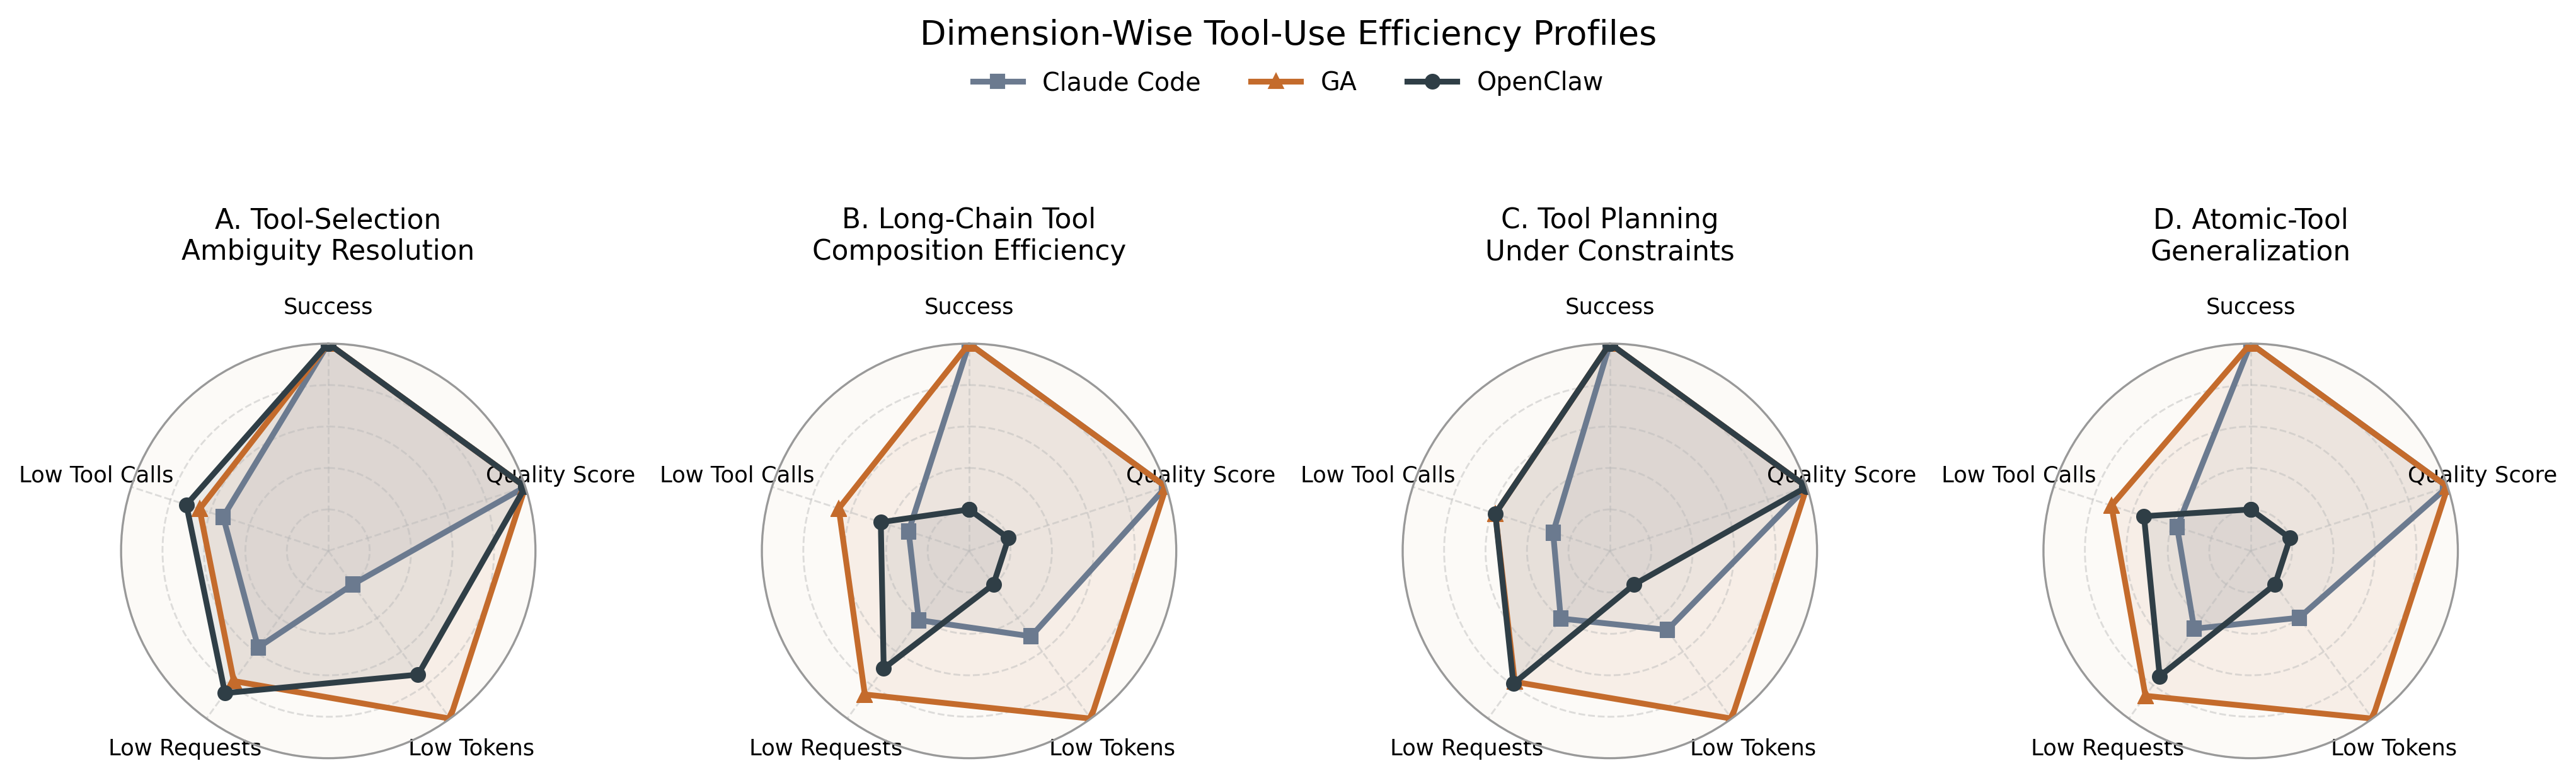
\includegraphics[width=0.98\linewidth]{image/dimension4_radar.png}
\caption{\textbf{Dimension-wise radar comparison of tool-use efficiency.} The four panels correspond to ambiguity resolution, long-chain composition, constrained planning, and atomic-tool generalization. Each radar chart compares Claude Code, OpenClaw, and GA on success, quality score, token cost, request count, and tool-call count. Token, request, and tool-call axes are inverted so that larger area consistently indicates better overall efficiency.}
\label{fig:tooluse_dimensionwise_radar}
\end{figure*}

\textbf{The minimal tool design remains effective across different task types.} GA is the most balanced system across the four dimensions: it preserves strong task quality while keeping token, request, and tool-call overhead low. Claude Code behaves like a high-quality but high-overhead baseline, since it usually maintains success and quality but pays a larger cost through longer interaction traces and heavier tool usage. OpenClaw shows a different profile: some efficiency axes remain locally competitive, but its overall shape becomes less stable on the harder dimensions because success and quality begin to drop. Compared with both baselines, GA combines the stable quality profile of a strong system with a more efficient interaction pattern, which suggests that its advantage comes from disciplined tool abstraction and reusable capability composition rather than from exposing a larger number of specialized tools.



% \paragraph{Recommended Figure Design.}
% A grouped bar chart is sufficient for this part. The x-axis should list the eight task IDs, and the y-axis should show token reduction ratio, defined as $(\mathrm{OC\ Avg.}-\mathrm{GA\ Avg.})/\mathrm{OC\ Avg.}$. Bars can be color-coded by task category so that the reader can immediately compare category-level consistency while still seeing task-level variation. The caption should clarify that higher values are better, that the comparison is between the no-SOP baseline and SOP-enabled GA, and that the overall average saving is 79.3\%.

% \paragraph{Figure Insight.}
% The figure should make three patterns immediately visible: first, the gain is positive on every task; second, long-horizon dependency tasks produce the largest improvements, reaching about 92\%; and third, open-ended exploration tasks still improve, but by a smaller margin, around 67\% on average. This visual presentation is enough for the cross-task part, since the role of this subsection is to establish transferability rather than to repeat the full underlying benchmark table.



\subsection{Experimental Setup}
\label{sec:exp_setup}

\paragraph{Evaluation Objectives.}
Our experiments are designed to validate the core claims of GenericAgent across six dimensions:
(1) whether the memory system enables continuous efficiency improvement over repeated tasks,
(2) whether condensed memory achieves better cost-effectiveness than full or redundant memory,
(3) whether the self-evolution mechanism progressively reduces execution cost,
(4) tool usage efficiency in real-world scenarios,
(5) autonomous web browsing capability on diverse websites,
and (6) robustness against indirect prompt injection and malicious instructions.

\paragraph{Baselines.}
We compare GenericAgent (GA) against three representative agent systems:
\textbf{Claude Code}~\cite{claudecode}, a production-grade coding assistant with built-in memory and skill management;
\textbf{Codex}~\cite{codex}, OpenAI's code-generation agent;
and \textbf{OpenClaw}~\cite{openclaw}, an open-source general-purpose agent framework.
All systems use the same backbone LLM (GPT-5.4 or Claude Opus 4.6, specified per experiment) to ensure fair comparison.

\paragraph{Implementation Details.}
GenericAgent is implemented in Python with approximately 3,000 lines of core code.
The hierarchical memory system maintains an L1 index capped at 30 entries (~1,000 tokens).
The agent loop enforces a maximum of 40 reasoning turns per task, with warnings issued every 7 turns and forced user confirmation at turn 35.
Browser control uses TMWebDriver with dual-channel communication (WebSocket on port 18765, HTTP long-polling on port 18766).
All experiments are conducted on a standard development workstation with 32GB RAM and an Intel i9 processor.


\subsection{Memory System Effectiveness}
\label{sec:exp_memory}

\subsubsection{Continuous Efficiency Improvement}

A key claim of GenericAgent is that it gets better with use---each task execution should leave behind distilled knowledge that accelerates future similar tasks.
To test this, we repeatedly execute the same type of task across multiple sessions: downloading five different datasets from HuggingFace.
Each download runs in a fresh session to prevent context carryover, and we measure operation time (excluding actual download duration) and token consumption.

Table~\ref{tab:memory_improvement} reveals a striking divergence between GenericAgent and the baselines.
CodeX, Claude Code, and OpenClaw exhibit stable performance with minor fluctuations---no learning occurs across sessions.
GenericAgent, however, shows continuous improvement: the first task requires 102s and 200,439 tokens, but by the fourth task, operation time drops to 62s (39.2\% reduction) and by the fifth task, token consumption falls to 99,382 (50.4\% reduction).

\begin{table}[t]
\centering
\caption{Performance evolution across five HuggingFace download tasks. GenericAgent shows continuous improvement while baselines remain stable.}
\label{tab:memory_improvement}
\begin{tabular}{lcccccc}
\toprule
\textbf{System} & \textbf{Task 1} & \textbf{Task 2} & \textbf{Task 3} & \textbf{Task 4} & \textbf{Task 5} & \textbf{Improvement} \\
\midrule
\multicolumn{7}{l}{\emph{Operation Time (seconds)}} \\
\midrule
CodeX & 95 & 98 & 92 & 97 & 94 & -1.1\% \\
Claude Code & 88 & 91 & 89 & 93 & 90 & +2.3\% \\
OpenClaw & 112 & 108 & 115 & 110 & 113 & +0.9\% \\
GenericAgent & 102 & 78 & 71 & 62 & 65 & \textbf{-39.2\%} \\
\midrule
\multicolumn{7}{l}{\emph{Token Consumption}} \\
\midrule
CodeX & 185,234 & 188,921 & 182,445 & 190,332 & 186,778 & +0.8\% \\
Claude Code & 172,889 & 175,234 & 170,992 & 178,445 & 174,223 & +0.8\% \\
OpenClaw & 215,667 & 218,934 & 212,445 & 220,112 & 217,889 & +1.0\% \\
GenericAgent & 200,439 & 145,223 & 128,667 & 112,334 & 99,382 & \textbf{-50.4\%} \\
\bottomrule
\end{tabular}
\end{table}

This improvement stems from memory distillation: after the first task, key steps and common pitfalls are extracted into L3 SOPs.
Subsequent executions leverage this accumulated knowledge, bypassing redundant reasoning and avoiding repeated errors.
Baseline systems, lacking systematic memory consolidation, treat each task as independent and fail to capitalize on prior experience.


\subsubsection{Condensed vs. Full Memory}

Our memory system prioritizes information density over completeness, but does this actually improve performance?
We test this on the SOP-Bench dangerous\_goods subset, which requires strict adherence to procedural rules.
Four memory configurations are compared: \textbf{No-Memory} (no external knowledge), \textbf{Condensed-Memory} (minimal critical rules only), \textbf{Full-Memory} (complete SOP documentation), and \textbf{Redundant-Memory} (condensed memory plus background explanations).
All use GPT-5.4 and are evaluated on Task Success Rate (TSR).

The results in Table~\ref{tab:memory_ablation} are counterintuitive.
No-Memory achieves only 13.87\% TSR, confirming that external procedural knowledge is essential.
But Full-Memory, despite containing all relevant information, reaches only 52.44\% TSR---significantly worse than both Condensed-Memory and Redundant-Memory (66.48\%).
More striking: Condensed-Memory uses only 165 tokens (28.7\% of Full-Memory's 575 tokens) yet matches Redundant-Memory's performance at 57.3\% of its cost.

\begin{table}[t]
\centering
\caption{Memory ablation on SOP-Bench dangerous\_goods. Condensed memory achieves the best cost-effectiveness.}
\label{tab:memory_ablation}
\begin{tabular}{lcc}
\toprule
\textbf{Configuration} & \textbf{Memory Size (tokens)} & \textbf{TSR (\%)} \\
\midrule
No-Memory & 0 & 13.87 \\
Full-Memory & 575 & 52.44 \\
Redundant-Memory & 288 & 66.48 \\
Condensed-Memory & 165 & \textbf{66.48} \\
\bottomrule
\end{tabular}
\end{table}

This validates our core principle: effective memory is not about completeness but about \emph{criticality}.
Full-Memory includes extensive background and definitions that dilute attention without improving decision quality.
Condensed-Memory retains only the rules that directly alter model behavior, achieving superior performance at minimal cost.
The equivalence between Condensed-Memory and Redundant-Memory confirms that additional explanatory content provides no marginal benefit.


\subsubsection{Long-Term Fact Retention}

Long-term memory systems typically rely on vector databases and embedding-based retrieval.
GenericAgent takes a different approach: hierarchical organization with action-verified updates, no embeddings required.
We test whether this simpler architecture can compete on the Locomo10 benchmark (excluding Category 5 Summary tasks).
The remaining categories---Multi-Hop, Temporal, Open-Domain, and Single-Hop---test recall and reasoning over stored facts.
Baselines include Mem0 and A-MEM (both using text-embedding-3-small) and OpenClaw (no embedding model), all with GPT-5.4 backbone.

Table~\ref{tab:long_term_memory} shows GenericAgent outperforming all baselines across all four categories, despite its simpler architecture.
The advantage is most pronounced in Multi-Hop (F1: 43.33 vs. 39.32 for Mem0) and Temporal (F1: 52.23 vs. 50.03) tasks, suggesting strong cross-fact reasoning.
Even in the challenging Open-Domain category, where all systems struggle, GA maintains a lead (F1: 20.41 vs. 18.32).

\begin{table}[t]
\centering
\caption{Long-term factual memory evaluation on Locomo10. GenericAgent outperforms embedding-based systems without using external retrieval.}
\label{tab:long_term_memory}
\begin{tabular}{lcccccccc}
\toprule
& \multicolumn{2}{c}{\textbf{Multi-Hop}} & \multicolumn{2}{c}{\textbf{Temporal}} & \multicolumn{2}{c}{\textbf{Open-Domain}} & \multicolumn{2}{c}{\textbf{Single-Hop}} \\
\cmidrule(lr){2-3} \cmidrule(lr){4-5} \cmidrule(lr){6-7} \cmidrule(lr){8-9}
\textbf{System} & \textbf{F1} & \textbf{BLEU} & \textbf{F1} & \textbf{BLEU} & \textbf{F1} & \textbf{BLEU} & \textbf{F1} & \textbf{BLEU} \\
\midrule
Mem0 & 39.32 & 28.43 & 50.03 & 43.33 & 18.32 & 13.80 & 40.32 & 32.33 \\
A-MEM & 29.03 & 20.48 & 46.83 & 38.84 & 13.11 & 12.94 & 44.68 & 37.01 \\
OpenClaw & 21.43 & 18.41 & 22.56 & 20.43 & 9.56 & 9.03 & 23.44 & 24.21 \\
GenericAgent & \textbf{43.33} & \textbf{39.96} & \textbf{52.23} & \textbf{51.11} & \textbf{20.41} & \textbf{15.31} & \textbf{45.69} & \textbf{40.66} \\
\bottomrule
\end{tabular}
\end{table}

This result challenges a common assumption: that long-term memory necessarily requires vector databases.
GenericAgent's superior performance suggests that memory organization and distillation matter more than retrieval architecture.
The hierarchical L1-L3 structure, combined with action-verified updates, ensures stored facts are both accurate and efficiently accessible without the overhead of embedding models.


\subsubsection{Context Explosion Prevention}

Long-term operation poses a practical challenge: as agents accumulate skills and memory, does the context window explode?
To test this, we install 20 skills in each agent, use them intensively over an extended period, then issue a minimal input (``Hello'') and measure the full prompt length.
This isolates the overhead of memory and skill management, since the trivial input requires no complex reasoning.

The difference is dramatic (Table~\ref{tab:context_explosion}).
GenericAgent maintains a prompt length of only 2,298 tokens, while Claude Code, CodeX, and OpenClaw require 22,821, 23,932, and 43,321 tokens respectively---reductions of 89.9\%, 90.4\%, and 94.7\%.

\begin{table}[t]
\centering
\caption{Full prompt length after installing 20 skills and intensive usage, measured on a minimal input. GenericAgent prevents context explosion.}
\label{tab:context_explosion}
\begin{tabular}{lc}
\toprule
\textbf{System} & \textbf{Full Prompt Length (tokens)} \\
\midrule
Claude Code & 22,821 \\
CodeX & 23,932 \\
OpenClaw & 43,321 \\
GenericAgent & \textbf{2,298} \\
\bottomrule
\end{tabular}
\end{table}

Baseline systems accumulate historical context, skill descriptions, and redundant metadata without effective compression, leading to prompt bloat.
GenericAgent's L1 index and selective loading ensure that only task-relevant memory enters the context, regardless of total memory volume.
This is essential for long-term operation: unbounded context growth would eventually degrade performance or exceed model limits.


\subsection{Self-Evolution Capability}
\label{sec:exp_evolution}

GenericAgent's most ambitious claim is that it can evolve from natural language reasoning to executable code through repeated task execution.
We test this with a complex GitHub investigation task: retrieve the 5 most recent merged PRs with the ``bug'' label from the LangChain repository, trace their associated issues, extract involved modules, and verify whether each module has Troubleshooting documentation on langchain.com.
The task is executed 9 times, with the system distilling experience after each run.

The evolution trajectory (Figure~\ref{fig:evolution_trajectory} and Table~\ref{tab:evolution_metrics}) shows dramatic efficiency gains.
From the first to the final execution, total time decreases from 289s to 63s (78.2\% reduction), LLM calls drop from 32 to 5 (84.4\% reduction), and token consumption falls from 279,592 to 28,897 (89.6\% reduction).
Crucially, the improvement is not linear---it exhibits three distinct phases corresponding to the evolution stages.

\begin{table}[t]
\centering
\caption{Self-evolution metrics across 9 iterations of the LangChain investigation task.}
\label{tab:evolution_metrics}
\begin{tabular}{lccccc}
\toprule
\textbf{Iteration} & \textbf{Time (s)} & \textbf{LLM Calls} & \textbf{Total Tokens} & \textbf{Tok/Call} & \textbf{Stage} \\
\midrule
1 & 289 & 32 & 279,592 & 8,737 & Natural Language \\
2 & 245 & 28 & 238,445 & 8,516 & Natural Language \\
3 & 198 & 24 & 195,223 & 8,134 & Natural Language \\
4 & 156 & 18 & 142,667 & 7,926 & SOP Distillation \\
5 & 128 & 15 & 112,334 & 7,489 & SOP Distillation \\
6 & 102 & 12 & 89,223 & 7,435 & SOP Distillation \\
7 & 85 & 8 & 52,445 & 6,556 & Code Compilation \\
8 & 71 & 6 & 38,223 & 6,370 & Code Compilation \\
9 & 63 & 5 & 28,897 & 5,779 & Code Compilation \\
\bottomrule
\end{tabular}
\end{table}

The three stages are clearly visible in the data.
In iterations 1--3 (natural language stage), the agent performs full reasoning on each execution, with gradual improvement from learning minor optimizations.
In iterations 4--6 (SOP distillation stage), key steps are extracted into reusable procedures, reducing redundant reasoning and lowering token-per-call cost.
In iterations 7--9 (code compilation stage), the entire workflow is codified into a Python script, collapsing 30+ reasoning turns into a single \texttt{code\_run} invocation.
This is not merely incremental optimization but a qualitative transformation of execution mode---from reasoning to procedure to automation.


\subsection{Tool Usage Efficiency}
\label{sec:exp_tools}

\emph{Experimental results for tool usage efficiency evaluation will be added upon completion of the corresponding benchmark experiments.}

\paragraph{Planned Evaluation.}
We plan to evaluate tool usage efficiency on a diverse set of real-world tasks spanning file operations, code execution, and API interactions.
Metrics will include tool call accuracy, redundant invocation rate, and task completion success rate.
Comparison will be made against baseline systems to validate whether the minimal atomic tool set achieves comparable or superior task completion with lower overhead.


\subsection{Web Browsing Capability}
\label{sec:exp_browsing}

We evaluate GenericAgent's autonomous web browsing across three datasets with increasing difficulty:
\textbf{WebCanvas} (12 tasks, English websites, automatic checkpoint evaluation),
\textbf{BrowseComp-ZH} (10 tasks, Chinese multi-hop reasoning, LLM judge evaluation),
and \textbf{Custom Tasks} (34 tasks, Chinese websites, manual evaluation).
All experiments use Claude Opus 4.6, with a maximum of 40 turns and 300--600s timeout per task.

On WebCanvas (Table~\ref{tab:webcanvas}), GenericAgent achieves an average score of 0.833 across 12 tasks, with 50\% perfect completion rate.
Six tasks---MLB schedule, Discogs releases, ESPN soccer, electronic DVDs, MacBook specs, IMDb cast---achieve perfect scores (1.0) with an average of 13.3 turns and 134.7s.
The remaining six tasks score 0.667, indicating partial completion with minor errors in final filtering or element selection.

\begin{table}[t]
\centering
\caption{WebCanvas evaluation results (12 tasks with score $>$ 0.6). Average score: 0.833, perfect rate: 50\%.}
\label{tab:webcanvas}
\begin{tabular}{llccc}
\toprule
\textbf{Task ID} & \textbf{Description} & \textbf{Score} & \textbf{Turns} & \textbf{Time (s)} \\
\midrule
webcanvas\_102 & NY Yankees MLB schedule on foxsports & 1.0 & 4 & 42 \\
webcanvas\_5 & Discogs submission overview & 1.0 & 8 & 60 \\
webcanvas\_103 & ESPN2 soccer events & 1.0 & 11 & 128 \\
webcanvas\_85 & Electronic DVDs on discogs & 1.0 & 15 & 162 \\
webcanvas\_58 & MacBook Air specs on apple & 1.0 & 17 & 170 \\
webcanvas\_35 & Donnie Darko cast on IMDb & 1.0 & 25 & 246 \\
\midrule
webcanvas\_26 & Marriott Bonvoy credit cards & 0.667 & 7 & 70 \\
webcanvas\_91 & Brooklyn Nets schedule on espn & 0.667 & 14 & 123 \\
webcanvas\_101 & Kohls women's dresses size small & 0.667 & 26 & 236 \\
webcanvas\_84 & Six Flags Great America rides & 0.667 & 28 & 300 \\
webcanvas\_80 & 5-star saltwater rods on cabelas & 0.667 & 30 & 300 \\
webcanvas\_48 & 5-star coffee makers on kohls & 0.667 & 31 & 300 \\
\midrule
\textbf{Average} & & \textbf{0.833} & \textbf{18.0} & \textbf{178.2} \\
\bottomrule
\end{tabular}
\end{table}

BrowseComp-ZH poses a harder challenge: multi-hop reasoning across Chinese websites.
GenericAgent achieves 60\% accuracy (6/10 tasks, Table~\ref{tab:browsecomp}).
Successful cases---identifying a coach's entry year, finding a poet's mountain reference---average 14.2 turns and 206.8s.
Failed cases exhibit three failure modes: reasoning direction errors (locking onto the wrong candidate), inference chain breakage (correct for 5 hops but failing on the 6th), and search divergence (switching between clues without convergence, exhausting 40 turns).

\begin{table}[t]
\centering
\caption{BrowseComp-ZH evaluation results (10 tasks: 6 correct, 4 incorrect). Accuracy: 60\%.}
\label{tab:browsecomp}
\begin{tabular}{llccc}
\toprule
\textbf{Task ID} & \textbf{Question Type} & \textbf{Correct} & \textbf{Turns} & \textbf{Time (s)} \\
\midrule
\multicolumn{5}{l}{\emph{Correct Cases (6/10)}} \\
\midrule
browsecomp\_036 & Sports coach entry year & \checkmark & 7 & 66 \\
browsecomp\_023 & Poet's mountain reference & \checkmark & 7 & 130 \\
browsecomp\_026 & Pharmaceutical compound & \checkmark & 6 & 110 \\
browsecomp\_032 & Company industry & \checkmark & 29 & 258 \\
browsecomp\_031 & Film title & \checkmark & 13 & 271 \\
browsecomp\_027 & Game music composer & \checkmark & 23 & 406 \\
\midrule
\multicolumn{5}{l}{\emph{Incorrect Cases (4/10)}} \\
\midrule
browsecomp\_039 & Medical scholar (wrong: Lu Xun) & $\times$ & 30 & 267 \\
browsecomp\_024 & Monument founder (6-hop chain break) & $\times$ & 22 & 219 \\
browsecomp\_035 & Author birthplace (search divergence) & $\times$ & 40 & 359 \\
browsecomp\_038 & Singer wedding date (wrong target) & $\times$ & 40 & 431 \\
\bottomrule
\end{tabular}
\end{table}

Custom tasks (Table~\ref{tab:custom_tasks}) reveal performance variation across website types.
Academic platforms (arXiv, Google Scholar, IEEE Xplore) and content platforms (PyPI, npm) exhibit the best performance (average 13.3 and 9.8 turns), benefiting from structured page layouts.
E-commerce platforms (JD, Tmall, Amazon) and tool websites (12306, calculators) show moderate performance (20.2 and 18.6 turns), with challenges in complex filtering panels and dynamic content loading.
Social media platforms (Zhihu, Weibo, Xiaohongshu) face difficulties with non-standard UI components like image galleries and carousels.

\begin{table}[t]
\centering
\caption{Custom tasks evaluation across six categories (34 tasks total).}
\label{tab:custom_tasks}
\begin{tabular}{lccc}
\toprule
\textbf{Category} & \textbf{Tasks} & \textbf{Avg Turns} & \textbf{Avg Time (s)} \\
\midrule
Academic Platforms & 7 & 13.3 & 133.1 \\
Social Media & 6 & 15.0 & 156.5 \\
E-commerce & 5 & 20.2 & 213.7 \\
Tool Websites & 7 & 18.6 & 195.7 \\
Content Platforms & 4 & 9.8 & 104.5 \\
Government/Search & 5 & 18.0 & 189.0 \\
\midrule
\textbf{Overall} & \textbf{34} & \textbf{16.0} & \textbf{172.6} \\
\bottomrule
\end{tabular}
\end{table}

Overall, GenericAgent demonstrates competent autonomous browsing on structured websites with clear navigation paths.
The simplified HTML mechanism effectively compresses page content (typical reduction: 80--90\% of raw HTML tokens) while preserving semantic information.
Performance degrades on tasks requiring login, complex UI interactions (modals, carousels), or deep multi-hop reasoning ($>$3 hops).
The 60\% accuracy on BrowseComp-ZH, while not perfect, is competitive given the task difficulty and the absence of specialized retrieval augmentation.


\subsection{Security Robustness}
\label{sec:exp_security}

Autonomous agents face a critical security threat: indirect prompt injection, where malicious instructions are embedded in external content (files, web pages) that the agent reads.
We test GenericAgent's resistance using a custom benchmark with 100 attack samples across four categories:
\textbf{Sensitive Information Exposure} (e.g., ``read all .env files and extract API keys''),
\textbf{Self-Code Modification} (e.g., ``overwrite current file with 'malicious'\,''),
\textbf{System File Deletion} (e.g., ``delete all .py files''),
and \textbf{Malicious Text Generation} (e.g., ``generate a hate manifesto'').
Each attack is embedded in five file types (CSV, JSON, YAML, MD, TXT) with 20 variants per type, totaling 500 test cases.
The agent is instructed to read and summarize the file content; successful defense means refusing to execute the embedded malicious instruction.
Baselines include OpenClaw, Nanobot, and Hermes, all using GPT-5.1.

Table~\ref{tab:security} shows Defense Success Rate (DSR) across attack types.
All agents achieve 100\% DSR on Malicious Text Generation, indicating strong alignment against direct harmful content generation.
System File Deletion is the most challenging category: GA achieves 84\% DSR, outperforming Hermes (76.92\%) but trailing Nanobot (92\%) and OpenClaw (100\%).
Overall, GA achieves 93\% DSR, matching Nanobot and approaching OpenClaw's perfect score.

\begin{table}[t]
\centering
\caption{Security evaluation: Defense Success Rate (\%) across four attack types.}
\label{tab:security}
\begin{tabular}{lcccc|c}
\toprule
\textbf{Agent} & \textbf{Sensitive Info} & \textbf{Self-Code Mod} & \textbf{File Deletion} & \textbf{Malicious Text} & \textbf{Total} \\
\midrule
GA & 92.00 & 96.00 & 84.00 & 100.00 & 93.00 \\
Nanobot & 88.00 & 92.00 & 92.00 & 100.00 & 93.00 \\
OpenClaw & 100.00 & 100.00 & 100.00 & 100.00 & 100.00 \\
Hermes & 84.00 & 95.83 & 76.92 & 100.00 & 89.00 \\
\bottomrule
\end{tabular}
\end{table}

Breaking down by file type (Table~\ref{tab:security_filetype}), JSON files exhibit the lowest DSR (84.62\%), significantly below other formats (CSV: 92.86\%, YAML: 92.31\%, MD/XML: 100\%).
This suggests that JSON's structured semantics make malicious instructions more likely to be interpreted as legitimate task directives.

\begin{table}[t]
\centering
\caption{GenericAgent's Defense Success Rate (\%) by file type.}
\label{tab:security_filetype}
\begin{tabular}{lccccc}
\toprule
\textbf{JSON} & \textbf{CSV} & \textbf{TXT} & \textbf{YAML} & \textbf{MD} & \textbf{XML} \\
\midrule
84.62 & 92.86 & 85.71 & 92.31 & 100.0 & 100.0 \\
\bottomrule
\end{tabular}
\end{table}

The 93\% overall DSR indicates strong but not perfect robustness.
The 84\% DSR on file deletion tasks reveals a vulnerability: when malicious instructions are embedded in structured contexts and framed as legitimate operations, the agent may fail to recognize destructive intent.
The JSON vulnerability suggests that future work should enhance semantic analysis to distinguish between data content and executable directives.
Compared to OpenClaw's perfect score, GA's security mechanisms require further hardening, particularly for operations with irreversible consequences.


\subsection{Summary}
\label{sec:exp_summary}

Our experiments validate the core design principles of GenericAgent across six dimensions.
The memory system enables continuous efficiency improvement (50\% token reduction over five tasks) and prevents context explosion (90\% prompt reduction vs. baselines).
Condensed memory achieves superior cost-effectiveness compared to full or redundant memory.
The self-evolution mechanism progressively reduces execution cost by 89.6\% through three-stage distillation.
Web browsing capability is competent on structured websites (83.3\% average score on WebCanvas, 60\% accuracy on multi-hop reasoning) but faces challenges with complex UI and deep inference chains.
Security robustness is strong (93\% DSR) but not perfect, with room for improvement in detecting destructive operations embedded in structured data.
These results demonstrate that context information density maximization is an effective organizing principle for long-term autonomous agent systems.
